\documentclass[notitlepage, 12pt]{article}
\usepackage[english]{babel}           % LANGEUAGE=ENGLISH, UTF-8
\usepackage[utf8]{inputenc}
\usepackage[T1]{fontenc}
\usepackage{amsmath}                  % ALL MATH FEATURES
\usepackage{graphicx}                 % GRAPHICS                  
\usepackage{float}                    % IMPROVED FIGURE POSITIONING
\usepackage[labelsep=period,labelfont=bf]{caption} % IMPROVED CAPTIONS
\usepackage{url}                      % WRITE URLS
\usepackage{tikz}                     % MAKE TIKZ VECTOR GRAPHICS
\usepackage{tocloft}                  % CONTROL TABLE OF CONTENTS
\usepackage[authoryear,round]{natbib} % REFERENCES
\usepackage{apalike}
\usepackage{pdflscape}                % USE LANDSCAPE MODE
\usetikzlibrary{decorations.pathreplacing}
\usepackage{enumitem}

\renewcommand{\familydefault}{lmr}           % SET DOCUMENT FONT
\makeatletter                         
\renewcommand{\section}{\@startsection       % SECTION
        {section}
        {2}
        {0mm}
        {1.2\baselineskip}
        {\baselineskip}
        {\centering\normalsize}}
\renewcommand{\subsection}{\@startsection    % SUBSECTION
        {subsection}
        {2}
        {0mm}
        {.8\baselineskip}
        {.5\baselineskip}
        {\bfseries\normalsize}}
\renewcommand{\subsubsection}{\@startsection % SUBSUBSECTION
        {subsubsection}
        {2}
        {0mm}
        {.5\baselineskip}
        {0mm}
        {\it\bfseries\normalsize}}
\makeatother
    
% define algorithm environments
\floatstyle{plaintop}
\newfloat{algorithm}{bpht}{alg}
\floatname{algorithm}{Algorithm}

%define title matter
\title{Simulating a dark matter halo using a parallel grid method}
\author{{\em Otto Hannuksela} \and {\em Janne Lampilahti}}
\date{\today}

\begin{document}
\maketitle
\section{INTRODUCTION}
Dark matter appears to be the dominant form of matter in the universe. While no direct observations of dark matter exist, it has been observed indirectly through its gravitational interaction with visible matter and radiation \citep{Roos2010}. The effect of dark matter on structure formation in the universe is the subject of an increasing scientific interest and a useful tool in the search for possible candidates of dark matter. Current progress in the investigation of structure formation is mainly driven by advances in computational methods and capabilities \citep{Kuhlen2012}. 

In this work we simulate a dark matter halo, neglecting baryonic matter, by using a particle based method and solving the Poisson's equation of gravity. The software used is {\em Uintah} (available from \url{http://uintah.utah.edu/} during the writing of this report), a parallel grid framework with a support for particle interactions and adaptive mesh refinement and which is aimed at solving partial differential equations. A major part of the project was to learn how to use the tools provided by Uintah.

\section{METHODS}

In this section the relevant theory and numerical methods are described. The method in short was to use a Poisson solver operating on a grid and an $N$-body integrator operating on particles, that are coupled via interpolation between the grid and the particles. This method is used in the context of massive collisionless particles interacting through gravity \citep[e.g.][]{Hockney1985}.  

%%%%%
\subsection{Theory}
A distribution of mass density $\rho$ gives rise to a gravitational potential $\phi$ according to the Poisson's equation of gravity
\begin{equation}
\nabla^2 \phi = 4\pi G \rho,
\end{equation}
where $G\approx 6.674\times10^{-11}$ Nm$^2$/kg$^2$ is the gravitational constant. In our simulation we normalize $G=1$. The corresponding force field can be solved from the gradient
\begin{equation}
\mathbf{F} = -\nabla \phi.
\end{equation}
In our simulation a distribution of massive particles create the mass density. A new position and velocity for the particles after a time step $dt$ can be solved from the Newton's equation of motion.
\begin{align}
\mathbf{v}(t+dt) &= \int_{t}^{t+dt}\frac{\mathbf{F}(t')}{m}dt' +  \mathbf{v}(t)\\
\mathbf{x}(t+dt) &= \int_{t}^{t+dt}\mathbf{v}(t')dt' +  \mathbf{x}(t)
\end{align}
The use of this theory assumes that we do not have relativistic speeds or masses and that the maximum grid size is small enough that expansion of the universe can be neglected.

One approach would be to try to calculate the particle-particle interactions but this is not computationally feasible since we would have $2^N$ interactions where $N$ is the particle number and we are using thousands of particles.  

%%%%%
\subsection{Numerical methods}\label{ssec:numerical}
The simulation is set up with respect to a three dimensional grid that supports particles (Fig. \ref{fig:grid}).
The overall algortihm is expressed in Algortihm \ref{alg:main}.
\begin{algorithm}[H]
\hspace{0.1\textwidth}\parbox{.8\textwidth}{
\-\hspace{0ex}set Dirichlet or periodic boundary conditions\\
\-\hspace{0ex}set initial $\mathbf{x}_p$, $\mathbf{v}_p$ and $m_p$ for all particles $p$\\
\-\hspace{0ex}interpolate initial $\rho$ from particle mass $m_p$\\
\-\hspace{0ex}set initial guess for $\phi$\\
\-\hspace{0ex}{\bf loop}\\
\-\hspace{4ex}solve $\phi$ at the nodes using the SOR algorithm\\
\-\hspace{4ex}calculate $\mathbf{F}=-\nabla \phi$ with respect to each particle $p$\\
\-\hspace{4ex}{\bf for} every particle $p$ {\bf do}\\
\-\hspace{8ex}$\mathbf{v}_p(t+\Delta t) = (\mathbf{F}_p/m)\Delta t + \mathbf{v}_p(t)$\\
\-\hspace{8ex}$\mathbf{x}_p(t+\Delta t) = \mathbf{v}_p(t)\Delta t + \mathbf{x}_p(t)$\\
\-\hspace{4ex}{\bf end for}\\
\-\hspace{4ex}interpolate new $\rho$ from particle mass $m_p$\\
\-\hspace{4ex}$t\leftarrow t+\Delta t$\\
\-\hspace{0ex}{\bf end loop}}
\caption{Main program.}
\label{alg:main}
\end{algorithm}

The Poisson's equation of gravity is discretized to 
\begin{equation}
\begin{aligned}
4\pi G\rho_{i,j,k} &= \frac{\phi_{i+1,j,k}-2\phi_{i,j,k}+\phi_{i-1,j,k}}{(\Delta x)^2}+\\
& \phantom{{}={}} \frac{\phi_{i,j+1,k}-2\phi_{i,j,k}+\phi_{i,j-1,k}}{(\Delta y)^2}+\\
& \phantom{{}={}} \frac{\phi_{i,j,k+1}-2\phi_{i,j,k}+\phi_{i,j,k-1}}{(\Delta z)^2}.
\end{aligned}
\end{equation}

The gravitational potential $\phi$ is then solved at each node using using the successive over-relaxation (SOR) algortihm (Algorithm \ref{alg:SOR}) . In the calculation of the potential gradient we obtain the potential values near the particles by interpolation and then calculate the gradient by numerical differentiation. For exmaple at the $p$th particle the gradient is calculated in the $x$ direction as
\begin{equation}
(\nabla \phi)(x_p)=\frac{\phi(x_p+dx)-\phi(x_p-dx)}{2dx},
\end{equation}
where $x_p$ is the particle's $x$ coordinate and $dx$ is a small distance.  

The particle velocity and position are evolved over a small time step $dt$, assuming that the force remains constant. Essentially this means calculating for each particle
\begin{align}
&=\mathbf{v}_p(t+\Delta t) = (\mathbf{F}_p/m)\Delta t + \mathbf{v}_p(t)\\
&=\mathbf{x}_p(t+\Delta t) = \mathbf{v}_p(t)\Delta t + \mathbf{x}_p(t).
\end{align}
After this using the new positions the particle masses are interpolated back to the nodes to obtain a new mass density $\rho$.

\begin{algorithm}[H]
\hspace{0.1\textwidth}\parbox{.8\textwidth}{
\-\hspace{0ex}{\bf function} SOR($\phi$, tolerance, max\_iterations)\\
\-\hspace{4ex}{\bf for} $n = 0,1,\ldots\mbox{max\_iterations}$ {\bf do}\\
\-\hspace{8ex}error $\sigma\leftarrow 0$\\
\-\hspace{8ex}{\bf for} every node $\phi_{i,j,k}$\\
\-\hspace{12ex}$\phi_{i,j,k}^{(n+1)} \leftarrow (1-\omega)\phi_{i,j,k}^{(n)} + \frac{\omega}{6} (\phi_{i+1,j,k}^{(n)} +\phi_{i-1,j,k}^{(n)}+$\\
\-\hspace{12ex}$\phantom{\phi_{i,j,k}^{(n+1)} \leftarrow }\phi_{i,j+1,k}^{(n)}+ \phi_{i,j-1,k}^{(n)} + \phi_{i,j,k+1}^{(n)} + \phi_{i,j,k-1}^{(n)} +$\\
\-\hspace{12ex}$\phantom{\phi_{i,j,k}^{(n+1)} \leftarrow} h^3\rho_{i,j,k})$\\
\-\hspace{12ex}update $\sigma$\\
\-\hspace{8ex}{\bf end for}\\
\-\hspace{8ex}{\bf if} $\sigma \leq $ tolerance, {\bf break}\\
\-\hspace{4ex}{\bf end for}\\
\-\hspace{4ex}{\bf return} $\phi$\\
\-\hspace{0ex}{\bf end function}}
\caption{Calculating potential $\phi$ using the SOR algorithm.}
\label{alg:SOR}
\end{algorithm}




%%%%%
\subsection{Initialization of the simultaion}
The specific case we want to study with our simulation is a dark matter halo. Dark matter halos are structures composed of dark matter, believed to envelope galaxy disks.

We randomly distribute dark matter particles into a box and let them collapse by the effect of gravity. We used either Dirichlet boundary conditions with $\rho=0$ or periodic boundary conditions.    

%%%%%
\subsection{Verification of results}
To verify the simulation results we test for energy conservation:
\begin{align}
T+V&=\mathrm{constant}\\
\frac{1}{2}\sum_{p} m_pv_p^2 + M\sum_{i,j,k}\phi_{i,j,k} &= \mathrm{constant} 
\end{align}
where $T$ is the total kinetic energy, $V$ is the total potential energy and $M$ refers to the total mass of the particles. In the context of gravitationl interactions only, the virial theorem is:
\begin{equation}
\langle T \rangle_\tau = -\frac{1}{2}\langle V \rangle_\tau
\end{equation}
where we take a time average of the kinetic and potential energy over a time period $\tau$.

We could not use time steps, distances or masses with proper units because the Uintah interpolator had some problems with large numerical values (see section \ref{ssec:uintah}). Therefore the set of values in our simulation have arbitrary units. To test energy conservation and virial theorem we solved a scaling factor $c$ from the virial theorem over some time interval $\tau_1$. The scaling factor relates the kinetic energy $T$ and potential energy $V$ of the system via $\langle T \rangle_{\tau_1}$=c$\langle V\rangle_{\tau_1}$.

Then we tested the virial theorem over some other time interval $\tau_2$ as well as energy conservation to see whether they are satisfied when we use the scaling factor $c$.  

We also compare the radial mass distribution of the obtained halo with the Navarro-Frenkel-White (NFW) profile, which is the radial mass distribution often obtained from simulations \citep{Navarro1995}. The profile is given by  
\begin{equation}
\rho(r) = \frac{\rho_0}{\frac{r}{R_s}\left(1 + \frac{r}{R_s}\right)^2},
\label{eq:nfw}
\end{equation}
where $r$ is distance from the center of the halo and $(\rho_0,R)$ are parameters.    

\section{IMPLEMENTATION}

In this section, we will often refer to Section \ref{ssec:numerical} and describe each numerical method's implementation in detail. During the whole 
project, we made a lot of effort to make sure the algorithms fit the Uintah framework. Because of this, we will have extensive description of 
the Uintah framework in the Section \ref{ssec:Uintah}, describing how the Uintah patches which are used in the Poisson solver work, 
how particle masses are interpolated to the grid and how the gradient of potential is calculated. 

Additionally, we will discuss some of the limitations and 
bugs of Uintah software which drained a painstaking amount of time from us. For more information on Uintah framework, please refer to the \emph{uintah\_presentation.pdf} 
we made on the software.

\subsection{Uintah} \label{ssec:Uintah}
% describe uintah

As mentioned in the title, we made a \emph{fully parallel} poisson solver utilizing particle-in-cell approach.

Before we start with the actual algorithms, let's go through the basics of Uintah. There are a few concepts to understand; \emph{cells}, \emph{patches}, 
\emph{ghost cells}, \emph{cell-centered variables}, \emph{node-centered variables}, \emph{face-centered variables} and \emph{particles}. 

We present an explanation for each of these accompanied by a Figure (Figure \ref{fig:grid}) demonstrating a visual description.

\begin{enumerate}
\item \emph{Cells} are finite boxes in the grid. These are the basic elements of our simulation. In the case of our poisson solver, we discretize our poisson equation 
based on cells in such a way that our discretization length \emph{h} in Equation \ref{eq:discretized_poisson} is the length between \emph{cells}.
\item \emph{Patches} are collections of \emph{cells} in our grid. The reason to have a concept of \emph{patches} is that Uintah uses patches to distribute 
workloads for different processes. In Uintah, whenever we iterate through \emph{cells}, we iterate through them patch-by-patch. This introduces some complications, 
such as how to handle the boundary between patches. The boundary issue will be further elaborated on.
\item \emph{Ghost cells} are cells which are one or more step beyond the border of a \emph{patch}. The whole concept of ghost cells is meaningless if we 
do not work in parallel. In a parallel simulation (employing more than one process), having ghost cells is of utmost importance because it is used to handle 
\emph{MPI communication} between different processes' \emph{patches}.
\item \emph{Cell-centered variables} are variables which are defined at the center of each \emph{cell}.
\item \emph{Node-centered variables} are variables which are defined at the corners of each \emph{cell}.
\item \emph{Face-centered variables} are variables which are defined at the faces of each \emph{cell}.
\item \emph{Particles} are point variables defined at any arbitrary point in the simulation grid. In our simulation, cell/node/face-centered variables 
interact with each other by interpolating particle variables to cell/node/face-centered positions and by interpolating cell/node/face-centered variables to 
particle positions.
\end{enumerate}

\begin{figure}[H]
\centering
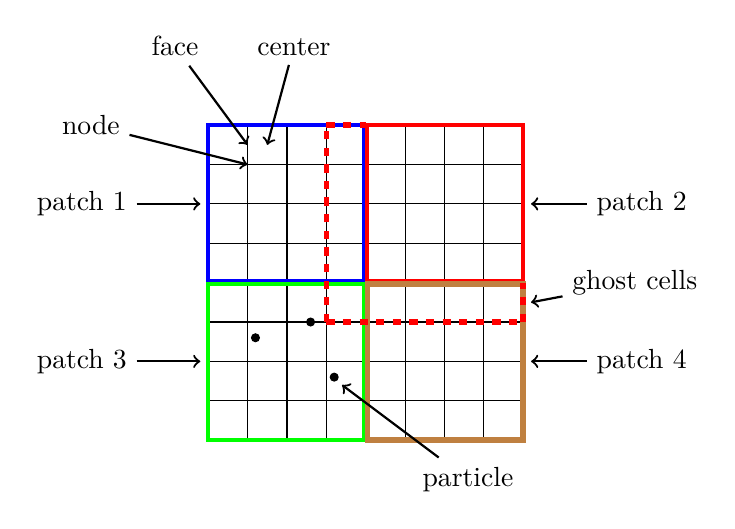
\begin{tikzpicture}
\node [anchor=east] (node) at (0,5) {node};
\node [anchor=east] (face) at (1,6) {face};
\node [anchor=west] (center) at (1.5,6) {center};
\node [anchor=west] (patch1) at (-1.3,4) {patch 1};
\node [anchor=east] (patch2) at (7.2,4) {patch 2};
\node [anchor=west] (patch3) at (-1.3,2) {patch 3};
\node [anchor=east] (patch4) at (7.2,2) {patch 4};
\node [anchor=east] (particle) at (5,0.5) {particle};
\node [anchor=west] (ghost) at (5.5,3) {ghost cells};
\draw [step=1] (1,1) grid (5,5);
\draw [step=0.5] (1,1) grid (5,5);
\draw [line width=1.5,color=blue] (1,3.02) rectangle (2.98,5);
\draw [line width=1.5,color=red] (3.02,3.02) rectangle (5,5);
\draw [line width=1.5,color=green] (1,1) rectangle (2.98,2.98);
\draw [line width=2,color=brown] (3.02,1) rectangle (5,2.98);
\draw [line width=2,color=red,dashed] (2.5,2.5) -- (5,2.5);
\draw [line width=2,color=red,dashed] (2.5,2.5) -- (2.5,5);
\draw [line width=2,color=red,dashed] (2.5,5) -- (3,5);
\draw [line width=2,color=red,dashed] (5,2.5) -- (5,3);
\draw [->,thick] (node) -- (1.5,4.5);
\draw [->,thick] (face) -- (1.5,4.75);
\draw [->,thick] (center) -- (1.75,4.75);
\draw [->,thick] (patch1) -- (0.9,4);
\draw [->,thick] (patch2) -- (5.1,4);
\draw [->,thick] (patch3) -- (0.9,2);
\draw [->,thick] (patch4) -- (5.1,2);
\draw [->,thick] (particle) -- (2.7,1.7);
\draw [->,thick] (ghost) -- (5.1,2.75);
\draw [fill] (2.3,2.5) circle [radius=0.05];
\draw [fill] (2.6,1.8) circle [radius=0.05];
\draw [fill] (1.6,2.3) circle [radius=0.05];
%\draw [black,decorate,decoration={brace,amplitude=5pt},
%   xshift=5pt,yshift=0pt] (5,5)  -- (5,3)
%   node [black,midway,below=-8pt,xshift=20pt] {AMR};
\end{tikzpicture}
\caption{A two dimensional view of the grid with its various components labeled.}
\label{fig:grid}
\end{figure}

Throughout our simulation, 



\subsection{The program}
\section{RESULTS}
\begin{figure}[H]
\centering
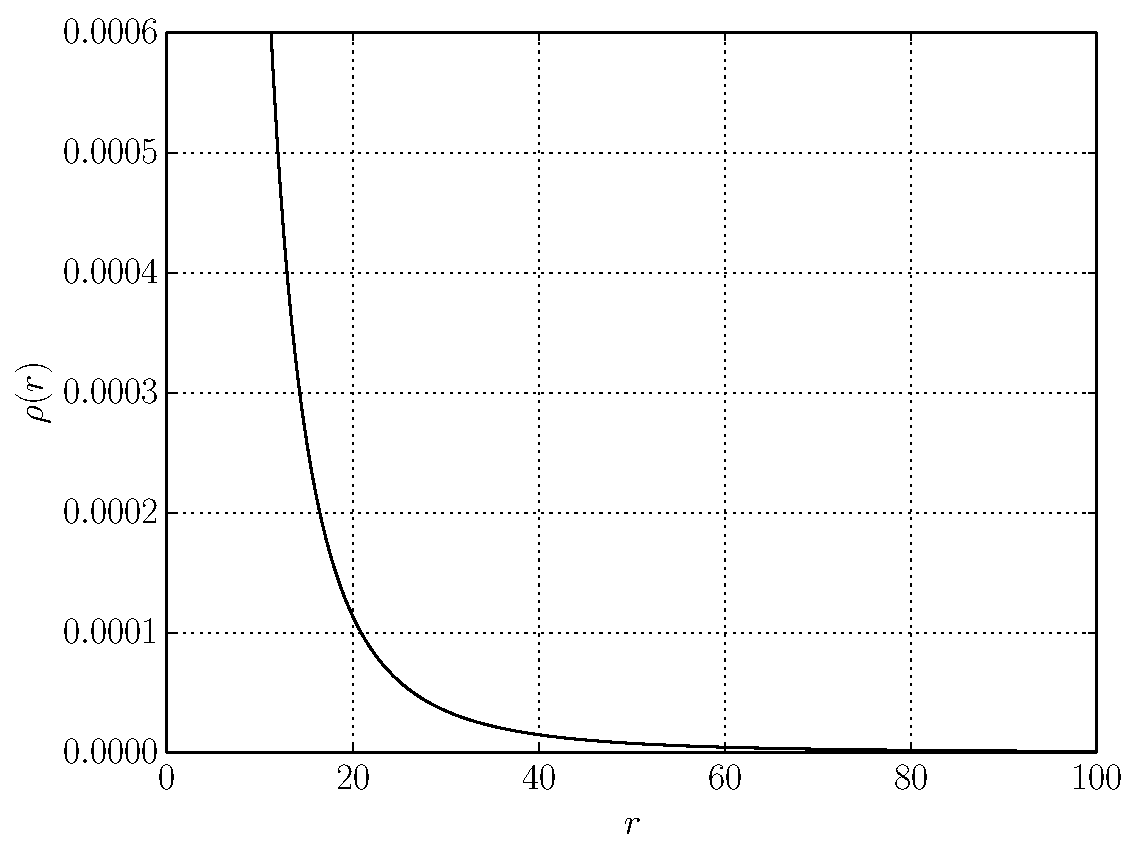
\includegraphics[width=.8\textwidth]{NFW_profile.pdf}
\caption{The shape of the radial distribution of mass density suggested by NFW profile (Equation \ref{eq:nfw}), choosing $\rho_0=1$ and $R_s=1$.}
\label{fig:nfw}
\end{figure}
% visit figure:
% initial vs final condition
% mp4 movie...
\section{CONCLUSIONS}
% what should we do next?

\renewcommand{\refname}{REFERENCES}
\begin{thebibliography}{}
\bibitem[Kuhlen et al., 2012]{Kuhlen2012}
Kuhlen, M. et al., (2012),
\newblock{Numerical Simulations of the Dark Universe: State of the Art and the Next Decade},
\newblock{arXiv:1209.5745 [astro-ph, physics:hep-ph]}
\bibitem[Roos, 2012]{Roos2010}
Roos, M., (2010),
\newblock{Dark Matter: The evidence from astronomy, astrophysics and cosmology},
\newblock{arXiv:1001.0316 [astro-ph]}
\bibitem[Hockeny and Eastwood, 1985]{Hockney1985}
Hockney, R.W. and Eastwood, J.W., (1985),
\newblock{Computer Simulation Using Particles},
\newblock{CRC Press}
\bibitem[Navarro et al., 1995]{Navarro1995}
Navarro, F.N. et al., (1995),
\newblock{The Structure of Cold Dark Matter Halos},
\newblock{arXiv:astro-ph/9508025}
\end{thebibliography}
\end{document}
